\documentclass{article}

\usepackage{blindtext}
\usepackage{graphicx}
\usepackage[skip=1ex]{caption}
\usepackage{subcaption}
\usepackage{amsmath}
\usepackage{amsfonts}
\usepackage{amssymb}
\usepackage{amstext}
\usepackage[english]{babel}
\usepackage{helvet}
\usepackage{microtype}
\usepackage[pdftex]{hyperref}
\usepackage{float}
\usepackage{xcolor}
\usepackage{tikz}
\usepackage{geometry}
\geometry{
    a4paper,
    left=2cm,
    right=2cm,
    top=1cm,
    bottom=1cm
}

\special{papersize=8.5in,11in}
\setlength{\pdfpageheight}{\paperheight}
\setlength{\pdfpagewidth}{\paperwidth}

% Macros

% Make inline frac bigger
\newcommand\ifrac[2]{{\displaystyle\frac{#1}{#2}}}

\begin{document}

\title{Written Assignment 0}

\author{Niraj Venkat}

\date{}

\maketitle

\vspace{.8cm}
\boxed{\text{Exercise} \quad 2.1}\\\\
\underline{Proving $\chi = V - E + F = 1$ for a polygonal disk:}
\\\\
If we start with a polygonal disk which has non-triangular faces, we can triangulate it by adding diagonals.
Each diagonal increases the number of edges and faces by 1. This process of triangulation leaves $\chi$ invariant.
\\
Now that all the faces are triangular, the remainder of the proof must show that $\chi = 1$. 
We start by removing triangles from the boundary which involves either:
\begin{itemize}
    \item Removing 1 face and 1 edge
    \item Removing 1 vertex, 2 edges and 1 face
\end{itemize}
Both would leave $\chi$ the same.
We are left with the base case which is just a triangle which has $\chi = 3 - 3 + 1 = 1$. 
\\\\
\underline{Proving $\chi = V - E + F = 2$ for a polygonal sphere:}
\\\\
We project the polyhedron to the 2D plane to re-use the previous result. To do this imagine shining a light from the top and casting a shadow 
on a surface placed on the bottom. This would yield a projection which has the same number of edges and vertices as before. 
If this is not the case, then we are allowed to reposition the vertices so that it casts a proper shadow. 
We are allowed to do this since $\chi$ is a topological property.
\\
The shadow we cast will have one less face than the original because that face is now the boundary of our shadow.
So $\chi = 1 + 1 = 2$ for the polygonal sphere.

\vspace{1.8cm}
\boxed{\text{Exercise} \quad 2.2}\\\\
\underline{Angles argument:}
\\
\begin{itemize}
    \item {\bfseries Triangles}. The interior angle of an equilateral triangle is 60 degrees. Thus on a regular polyhedron, only 3, 4, or 5 triangles can meet a vertex. If there were more than 6 their angles would add up to at least 360 degrees which they can't. Consider the possibilities:
    \begin{itemize}
        \item 3 triangles meet at each vertex, giving rise to a Tetrahedron
        \item 4 triangles meet at each vertex, giving rise to an Octahedron
        \item 5 triangles meet at each vertex, giving rise to an Icosahedron
    \end{itemize}
    \item {\bfseries Squares}. Since the interior angle of a square is 90 degrees, at most three squares can meet at a vertex. This is indeed possible and it gives rise to a hexahedron or cube.
    \item {\bfseries Pentagons}. As in the case of cubes, the only possibility is that three pentagons meet at a vertex. This gives rise to a Dodecahedron.
    \item {\bfseries Hexagons} or regular polygons with more than six sides cannot form the faces of a regular polyhedron since their interior angles are at least 120 degrees.
\end{itemize}
We end up with 5 platonic solids.
\\\\
\underline{Connectivity argument:}
\\\\
Because this is a regular polytope/mesh, the valence of each vertex is equal, so 
we argue each face is an identical $n$-gon, for some positive $n$.\\
Being regular implies $n \ge 3$.\\
With the same argument, each vertex is identical, so let $d$ be the degree of vertices.\\
Being regular implies $d \ge 3$.\\\\
As usual $V$ is number of vertices, $E$ is number of edges and $F$ is number of faces.\\
Each edge touches two faces, so $\ifrac{nF}{2} = E \implies F = \ifrac{2E}{n}$.\\
Each edge touches two vertices, so $\ifrac{dV}{2} = E \implies V = \ifrac{2E}{d}$.\\\\
Using Euler's formula:
\begin{equation}
    \begin{split}
    \chi = 2 &= V - E + F\\
             &= \frac{2E}{d} - E + \frac{2E}{n}\\
             &= E \, \Bigl(\frac2d - 1 + \frac2n \Bigr)
    \end{split}
    \notag
\end{equation}
From earlier $n \ge 3$ and $d \ge 3$, so we get $\ifrac1n \le \ifrac13$ and $\ifrac1d \le \ifrac13$.\\
$E$ must be positive so:
\begin{align}
    \frac2d - 1 + \frac2n > 0
    \notag
    \\
    \frac1d> \frac12 - \frac1n > \frac12 - \frac13 = \frac16
    \notag
    \\
    3 \le d < 6
    \notag
\end{align}
\\
When $d = 3$, $\ifrac1n > \ifrac16$, so $n = 3,\: 4 \: \text{or} \: 5$.\\\\
When $d = 4$, $\ifrac1n > \ifrac14$, so $n = 3$.\\\\
When $d = 5$, $\ifrac1n > \ifrac{3}{10}$, so $n = 3$.\\\\

Overall, this gives us the following table of platonic solids:

\begin{center}
    \begin{tabular}{ |c|c|c|c|c|c|c| } 
        \hline
        $d$ & $n$ & $V$ & $E$ & $F$ & Solid & Mesh \\ 
        \hline
        \hline
        3 & 3 & 4 & 6 & 4 & Tetrahedron & 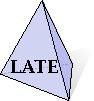
\includegraphics{figs/LatonicSolids/LateTetrahedron.pdf}\\ 
        \hline
        3 & 4 & 8 & 12 & 6 & Cube & 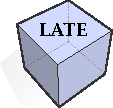
\includegraphics{figs/LatonicSolids/LateCube.pdf}\\ 
        \hline 
        3 & 5 & 20 & 30 & 12 & Dodecahedron & 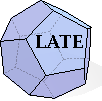
\includegraphics{figs/LatonicSolids/LateDodecahedron.pdf}\\ 
        \hline 
        4 & 3 & 6 & 12 & 8 & Octahedron & 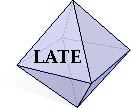
\includegraphics{figs/LatonicSolids/LateOctahedron.pdf}\\ 
        \hline 
        5 & 3 & 12 & 30 & 20 & Icosahedron & 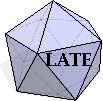
\includegraphics{figs/LatonicSolids/LateIcosahedron.pdf}\\ 
        \hline
\end{tabular}
\end{center}

The whole \lq LATE\rq \, thing is a joke that can be found \href{https://brickisland.net/DDGSpring2022/assignments/}{here}.

\pagebreak
\boxed{\text{Exercise} \quad 2.3}\\\\

Previous formulas apply here, with $n=3$ and $d=6$.
We apply the Euler-Poincaré formula:
\begin{equation}
    \begin{split}
    \chi = 2 - 2g   &= V - E + F\\
                    &= \frac{2E}{d} - E + \frac{2E}{n}\\
                    &= \frac{2E}{6} - E + \frac{2E}{3}\\
                    &= 0
    \end{split}
    \notag
\end{equation}
So we get $2(1-g) = 0 \implies g=1$, which is a torus.


\vspace{1.8cm}
\boxed{\text{Exercise} \quad 2.4}\\\\

Let the number of vertices with irregular valence be $n$.\\
The valences of these $n$ vertices are $v_1, v_2, \dots, v_n$, and we assume $v_i \ge 3$.
Using the previous formula for regular triangle mesh with degree $d$: $dV=2E=3F$.
This degree for irregular mesh is not uniformly $d$ so we now have:
\begin{align}
6(V-n)+\sum_i^n{v_i}=2E=3F
\notag\\
\implies F=\frac{6(V-n)+\sum_i^n{v_i}}{3}
\notag
\end{align}
We apply the Euler-Poincaré formula, and express in terms of $V$:
\begin{equation}
    \begin{split}
    \chi = 2 - 2g   &= V - E + F\\
                    &= V - \frac32 F + F\\
                    &= V - \frac12 F\\
                    &= V - \frac{6(V-n)+\sum_i^n{v_i}}{6}\\
                    &= n - \frac{\sum_i^n{v_i}}{6}\\
    \end{split}
    \notag
\end{equation}

So $n = 2 - 2g + \ifrac{\sum_i^n{v_i}}{6}$.
Because $v_i \ge 3$:
\begin{equation}
    \sum_i^n{v_i} \ge 3n
    \implies \frac{\sum_i^n{v_i}}{6} \ge \frac{n}{2}
    \implies n - 2 + 2g \ge \frac{n}{2}
    \implies n \ge 4 - 4g
    \notag
\end{equation}
\underline{When $g = 0$}: we have $n \ge 4$.\\\\
\underline{When $g = 1$}: we have $n = 0$ from Exercise 2.3\\\\
\underline{When $g \ge 2$}: we have $n \le -4$. \\
$n$ is non-negative, and if $n = 0 = 2\chi$, implies $\chi = 0$ for genus $g \ge 2$ which is invalid.
So the valid values start from $n \ge 1$.\\


Which gives us our result:
\begin{equation}
    m(K) =
\begin{cases}
    4, &g = 0\\
    0, &g = 1\\
    1, &g \ge 2\\
\end{cases}
\notag
\end{equation}


\pagebreak
\boxed{\text{Exercise} \quad 2.5}\\\\

\underline{Triangle mesh:}\\
Each edge has 2 faces on either side, each face is bounded by 3 edges. So $3F = 2E$ or $E:F = 3:2$.\\

We apply the Euler-Poincaré formula:\\

\begin{equation}
    \begin{split}
    \chi = 2 - 2g   &= V - E + F\\
                    &= V - E + \frac23 E\\
    \end{split}
    \notag
\end{equation}
\begin{equation}
    \implies E = 3(V-2+2g)
    \notag 
\end{equation}
An edge connects two vertices, but we can say that the edge belongs to only one of the vertices. So, mean valence for a triangle mesh of large V:\\
\begin{equation}
    \lim_{V\to\infty} \frac{2E}{V} = \lim_{V\to\infty} \frac{6(V-2+2g)}{V} = 6
    \notag
\end{equation}

\vspace{1.8cm}
\boxed{\text{Exercise} \quad 2.6}\\\\

\underline{Quad mesh:}\\
Very similar to the previous calculation, except each face is bounded by 4 edges, so $E:F = 4:2 = 2:1$.\\
We apply the Euler-Poincaré formula and get: $E = 2(V-2+2g)$

Mean valence for a quad mesh of large V:\\
\begin{equation}
    \lim_{V\to\infty} \frac{2E}{V} = 4
    \notag
\end{equation}

\vspace{1.8cm}
\boxed{\text{Exercise} \quad 2.7}\\\\

\underline{Tet mesh:}\\
TODO: find a proper explanation:\\
I found an explanation from \href{https://math.stackexchange.com/q/1879347}{Stack Exchange} which gives us the following result:\\
$$V:E:F:T = 1:4:6:3$$ \\
whereas the data included in the problem gives us something like:\\
$$V:E:F:T = 2:14:3:1$$ \\
So, I don't know what to make of this proof.\\
\par\noindent\rule{0.25\textwidth}{0.4pt}


Let $d$ be a positive integer and $M$ a $d$-dimensional triagularizable geometric object.  Let $F_j$ denote the number of $j$-dimensional faces of a triangularization $T$ of $M$.  (For example, $F_0$ is the number of vertices and $F_1$ is the number of edges.)  Each time a new vertex is added into the interior of an $n$-simplex in $T$, we see that the new triangularization $T'$ satisfies
$$
F_j'=
\begin{cases}
    F_j+\binom{d+1}{j}\,,&\text{ if }j=0,1,2,\ldots,d-1\,,\\
    F_d+d\,,&\text{ if }j=d\,,
\end{cases}
$$
where $F'_j$ is the number of $d$-dimensional faces in $T'$ for each $j=0,1,2,\ldots,d$.  Hence, if you refine the mesh on $M$ nicely (i.e., avoid fiddling with boundaries of all $n$-simplices), then the ratio
$$F_0:F_1:\ldots:F_{d-1}:F_d$$
should tend to
$$\binom{d+1}{0}:\binom{d+1}{1}:\ldots:\binom{d+1}{d-1}:d\,,$$
as the number of vertices increases.  In particular, for $d=3$, one would expect $$\frac{F_1}{F_0}\approx \frac{\binom{3+1}{1}}{\binom{3+1}{0}}=4\,.$$  If we are allowed to play with the boundaries of $n$-simplices, then the ratios $\frac{F_{j}}{F_{j-1}}$ for $j=1,2,\ldots,d$ may not have limits, or can tend to arbitrarily large values, provided that $d\geq 3$.

\vspace{1.8cm}
\boxed{\text{Exercise} \quad 2.8}\\\\

Luckily the mesh in this problem matches the one in the coding exercise!\\

% Putting two newlines after \hfill messes things up...

\begin{table}[ht]
    \begin{subfigure}{0.45\columnwidth}
    \includegraphics[width=\linewidth]{figs/2_8_orig.png}
    \caption{Original subset $\mathcal{S}$}
    \end{subfigure}\hfill
    %
    \begin{subfigure}{0.45\columnwidth}
    \includegraphics[width=\linewidth]{figs/2_8_star.png}   
    \caption{Star St($\mathcal{S}$)}
    \end{subfigure}\\[1em]
    %
    \begin{subfigure}{0.45\columnwidth}
    \includegraphics[width=\linewidth]{figs/2_8_closure.png}
    \caption{Closure Cl($\mathcal{S}$)}
    \end{subfigure}\hfill
    %
    \begin{subfigure}{0.45\columnwidth}
    \includegraphics[width=\linewidth]{figs/2_8_link.png} 
    \caption{Link Lk($\mathcal{S}$)}
    \end{subfigure}
\end{table}%



\pagebreak
\boxed{\text{Exercise} \quad 2.9}\\\\


\begin{table}[ht]
    \begin{subfigure}{0.45\columnwidth}
    \includegraphics[width=\linewidth]{figs/2_9_orig.png}
    \caption{Original subset $\mathcal{K}^\prime$}
    \end{subfigure}
    %
    \begin{subfigure}{0.45\columnwidth}
    \includegraphics[width=\linewidth]{figs/2_9_bd.png}   
    \caption{Boundary bd($\mathcal{K}^\prime$)}
    \end{subfigure}\\[1em]
    %
    \begin{subfigure}{0.45\columnwidth}
    \includegraphics[width=\linewidth]{figs/2_9_int.png}
    \caption{Interior int($\mathcal{K}^\prime$)}
    \end{subfigure}
\end{table}%



\vspace{1.8cm}
\boxed{\text{Exercise} \quad 2.10}\\\\


\underline{Twin}
\begin{center}
    \begin{tabular}{ c|c|c|c|c|c|c|c|c|c|c } 
        $h$&0&1&2&3&4&5&6&7&8&9\\
        \hline
        $\eta(h)$&4&2&1&5&0&3&7&6&9&8
    \end{tabular}
\end{center}

\underline{Next}
\begin{center}
    \begin{tabular}{ c|c|c|c|c|c|c|c|c|c|c } 
        $h$&0&1&2&3&4&5&6&7&8&9\\
        \hline
        $\rho(h)$&1&2&0&4&5&6&3&9&7&8
    \end{tabular}
\end{center}


\pagebreak
\boxed{\text{Exercise} \quad 2.11}\\\\

Looks like this:\\\\

\tikz 
\draw[thick]
  (0,0) -- (0,2) -- (2,2) -- (2,0) -- (0,2) -- (2,2) -- (0,0) -- (2,0);




\vspace{1.8cm}
\boxed{\text{Exercise} \quad 2.12}\\\\


\begin{align}
    A_0 = \begin{pmatrix}
        1 & 1 & 0 & 0 & 0\\
        1 & 0 & 1 & 0 & 0\\
        1 & 0 & 0 & 1 & 0\\
        1 & 0 & 0 & 0 & 1\\
        0 & 1 & 0 & 0 & 1\\
        0 & 1 & 1 & 0 & 0\\
        0 & 0 & 1 & 1 & 0\\
        0 & 0 & 0 & 1 & 1\\
    \end{pmatrix}
    \quad\quad
    A_1 = \begin{pmatrix}
        1 & 0 & 0 & 1 & 1 & 0 & 0 & 0\\
        1 & 1 & 0 & 0 & 0 & 1 & 0 & 0\\
        0 & 1 & 1 & 0 & 0 & 0 & 1 & 0\\
        0 & 0 & 1 & 1 & 0 & 0 & 0 & 1\\
    \end{pmatrix}
    \notag
\end{align}


\vspace{1.8cm}
\boxed{\text{Exercise} \quad 2.13}\\\\

For a simplicial $k-$manifold, the link of every vertex (0-simplex) looks like a $(k-1)-$dimensional sphere.\\
A simplicial $1-$complex is just a graph, but a simplicial $1-$manifold is not an arbitrary graph.\\
The degree of each vertex is no greater than 2, so the link of every vertex should be a pair of vertices.\\
So it cannot contain anything other than isolated paths of edges and closed loops of edges.



\vspace{1.8cm}
\boxed{\text{Exercise} \quad 2.14}\\\\

The boundary of a simplicial surface will have zero or more closed loops.\\
Each connected set of vertices with a boundary will generate a closed loop for its boundary.


\pagebreak
\boxed{\text{Exercise} \quad 2.15}\\\\

Here are a few ways to show that bd(bd($\mathcal{K}$)) = $\emptyset$:

\begin{itemize}
    \item
    Taking the boundary bd($\mathcal{K}$) means removing the interior: bd($\mathcal{K}$) = Cl($\mathcal{K}$) $\setminus$ int($\mathcal{K}$).
    We could say that int(bd($\mathcal{K}$)) = Cl(bd($\mathcal{K}$)) which gives us our result.
    
    \item
    Given a $k$-dimensional point set $\mathcal{K}$, for all points $p$ in the boundary of $\mathcal{K}$, the intersection of some
    open ball around $p$ is homeomorphic to an open $(k-1)$-ball.
    
    \item
    In DDG the boundary is defined as the closure of the set of all simplices $\sigma$ that are proper faces of exactly one simplex of $\mathcal{K}$. 
    The result of taking the boundary is a $(k-1)-$submanifold without any proper faces of exactly one simplex.
    This means $\sigma$ for bd($\mathcal{K}$) becomes $\emptyset$.
    \begin{center}
        bd(bd($\mathcal{K}$)) = Cl($\sigma$) = Cl($\emptyset$) = $\emptyset$.
    \end{center}
\end{itemize}























\end{document}
